\subsection{Multi-project}
\begin{frame}{Management of the multi-project}
	The multi-project consists of
	\begin{description}
		\item[Students:]{60}
		\item[Groups:]{16}
	\end{description}

	Development method: Scrum
	\begin{description}
		\item[Sprints]{Project split into four sprints}
		\begin{itemize}
			\item[Sprint 1] 24-02-2014 -- 19-03-2104 
			\item[Sprint 2] 20-03-2014 -- 14-04-2104
			\item[Sprint 3] 15-04-2014 -- 07-05-2104
			\item[Sprint 4] 08-05-2014 -- 27-05-2104
		\end{itemize}
	\end{description}
\end{frame}

\begin{frame}{Roles and responsibilities}
	Roles assigned on multi-project level and their responsibilities
	\begin{description}
		\item[Scrum Master] Chairing Scrum meetings and coordination of groups and meetings.
		\item[Sprint End Specialist] Coordinator and chairman of sprint review meetings.
		\item[Client Contact] Responsible for all communication to and from the clients.
	\end{description}
\end{frame}

\subsection{Structure}
\begin{frame}{Structure of the multi-project}
\begin{columns}
\begin{column}{.38\textwidth}
\begin{itemize}
\item Using scrum on 16 groups requires Scrum of Scrums
\item One meeting each week, for all groups
\end{itemize}
\end{column}
\begin{column}{.58\textwidth}
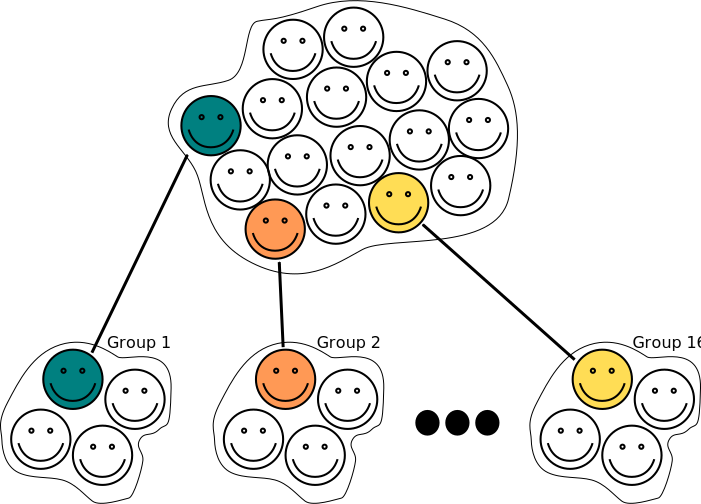
\includegraphics[width=\textwidth]{pres/scrumofscrums}
\end{column}
\end{columns}
\end{frame}

\subsection{Graphical Interface Resources for Autistic Folk (GIRAF)}
\begin{frame}{Project overview}
	\begin{itemize}
		\item<1> The purpose of GIRAF
		\item<2> Collection of front-end and back-end applications
		\item<3> The goals of the semester for GIRAF
		\begin{center}
		\includegraphics<2>[width=0.8\textheight]{pres/girafstructure}
		\end{center}
	\end{itemize}
\end{frame}

\subsection{The Launcher Project}
\begin{frame}{Launcher}
	\begin{description}
		\item<1>[What is Launcher]{An application launcher}
		\includegraphics<1>[width=0.8\textheight]{pres/launcherdescription}
		\item<2>[Permissions] Restriction of access to the android system
		\item<3>[Users] Management of users
	\end{description}
\end{frame}

\begin{frame}{Structure}
	\center
	\begin{center}
		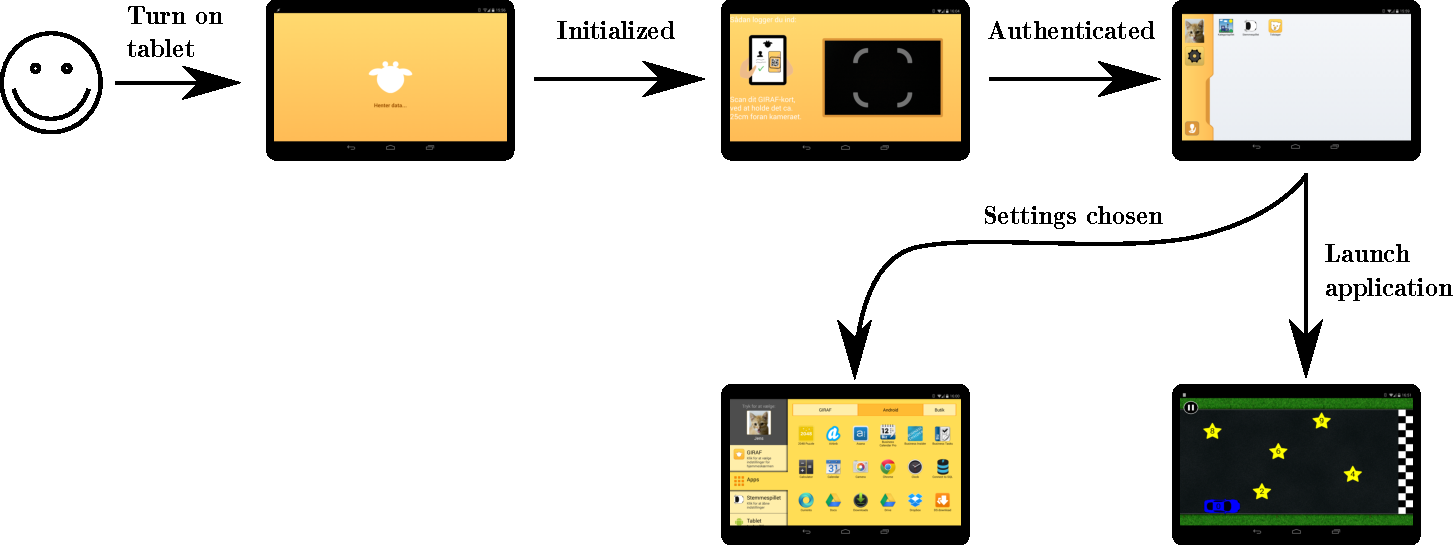
\includegraphics[width=\textwidth]{pres/launcherstructure}	
	\end{center}
\end{frame}